\section{Results}
\label{sec:results}

%% FIGURE: Koopman simulation plot
\begin{figure}
    \centering
    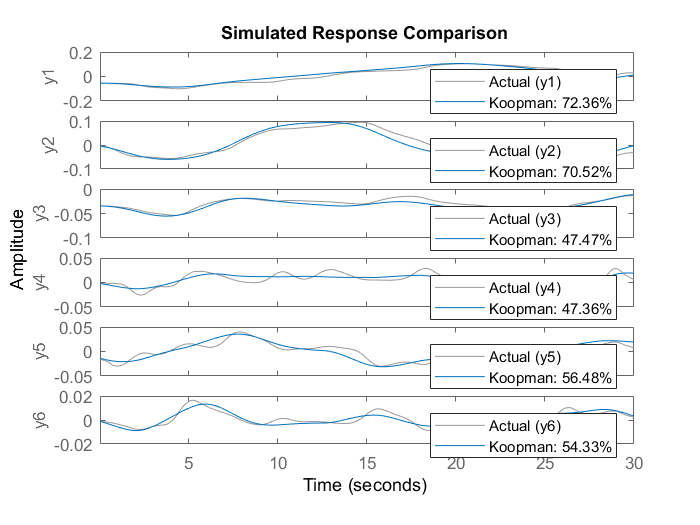
\includegraphics[width=\linewidth]{figures/koopPlot_ph1.png}
    \caption{PLACEHOLDER: Simulation of model generated by Koopman system identification technique verses real system.
    Simulation of the model generated by the Koopman sysid method (blue) superimposed with the measured behavior of the system (grey) over a 30 second time window given the same initial condition and control inputs. The NRMSE for each state is shown in the boxes on the right. \Ram{Please label the y-axis in each plot appropriately. It maybe worth comparing at least one other prediction generated from another sys id technique. Please color everything the same way, consistently (e.g. blue is Koopman, purple is n.n., etc.). Given space restrictions we may want to show another prediction as well. I'd remove the NRMSE from the plot. }}
    \label{fig:koopmanSim}
\end{figure}

%% Performance was evaluated by comparing simulations to real measurements
A state space model was generated from the technique described in section \ref{sec:theory} using a monomial basis of maximum degree $w=3$.
We evaluated its accuracy by comparing model simulations to validation data (Fig. \ref{fig:koopmanSim}).
Goodness of fit for the trajectory of a state $y$ was calculated using the normalized root-mean-square error (NRMSE)
%% Normalized Root Mean-Square Error
\aln{
    \text{NRMSE} &= \frac{\text{RMSE}}{y_\text{max} - y_\text{min}} \\
    \text{RMSE} &= \sqrt{ \frac{\sum_{k=1}^{N_\text{total}} \left( y_k - \hat{y}_k \right)^2}{N_\text{total}} }
    % 1 - \frac{ \| y - \hat{y}  \| }{ \| y - \text{mean}(y) \| }
}
where $\hat{y}$ is the simulated value of the state, $N_\text{total}$ is the total number of points, and $y_{\text{min/max}}$ are the measured maximum/minimum values of the state observed over all trials.
% A NRMSE of $1$ denotes a perfect fit, while a value less than or equal to $0$ implies that the model output is no better than a straight line at fitting the validation data.

%% For comparison, other sysid methods were also used on the same set of data
The performance of our model was benchmarked against several other models that were generated using the Matlab System Identification Toolbox and Neural Network Toolbox \cite{MATLAB:2017}.
These models were trained on the same data set as the Koopman model, 
Then, the models were simulated under the same inputs as those from the validation trials described in section \ref{sec:experiment}.
Fig. \ref{fig:comparison} shows the NRMSE of each model over all states and all trials as compared to the validation data.
The Koopman model exhibits a lower NRMSE than all of the other methods as well as a smaller standard deviation of error.
This implies that the Koopman model captures the real behavior of the system better and more consistently than the other models.

%% Why does Koopman model do better
There are several reasons why the performance of the Koopman model may be superior to the other models.
Since the Koopman model is a state space model, it is possible to initialize the model from the same initial condition as the real system.
This is not the case for the neural network and NLARX, which serve as black-box models which can only accept inputs and map them to outputs, without a notion of internal system state.
\Dan{I need to read up a little on how some of these methods work to offer a more thourough argument here...}.

%% FIGURE: Comparison bar graph
\begin{figure}
    \centering
    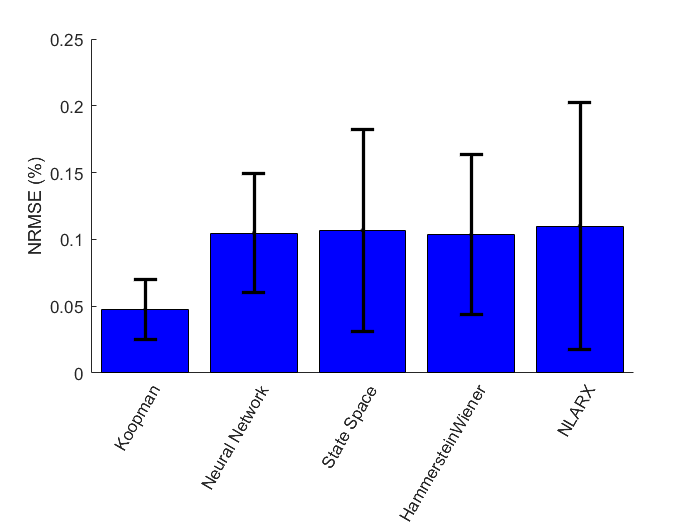
\includegraphics[width=\linewidth]{figures/bar_ph2.png} \\
    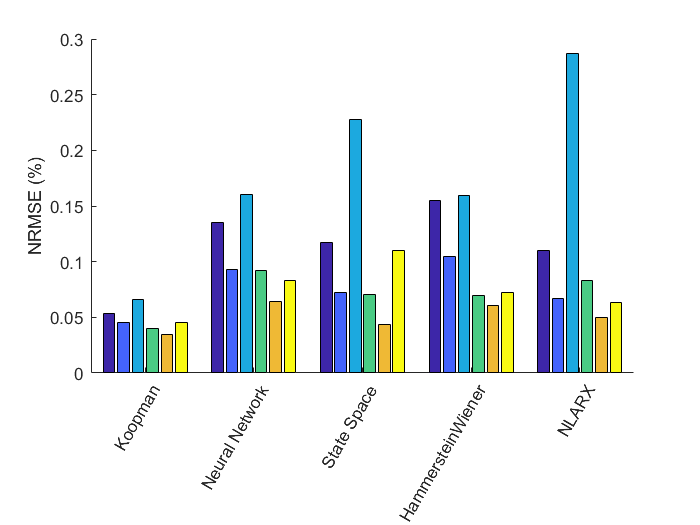
\includegraphics[width=\linewidth]{figures/barStates_ph1.png}
    \caption{PLACEHOLDER: The average NRMSE across all states and all trials for each model (top). The average NRMSE across all trials for each state within each model (bottom).}
    \label{fig:comparison}
\end{figure}